%%%%%%%%%%%%%%%%%%%%%%%%%%%%%%%%%%%%%%%%%
% Beamer Presentation
% LaTeX Template
% Version 1.0 (10/11/12)
%
% This template has been downloaded from:
% http://www.LaTeXTemplates.com
%
% License:
% CC BY-NC-SA 3.0 (http://creativecommons.org/licenses/by-nc-sa/3.0/)
%
%%%%%%%%%%%%%%%%%%%%%%%%%%%%%%%%%%%%%%%%%

%----------------------------------------------------------------------------------------
%	PACKAGES AND THEMES
%----------------------------------------------------------------------------------------

\documentclass{beamer}
\usepackage{pgfpages}
\usepackage{colortbl}
\usepackage{booktabs}
\usepackage{multirow}
\usepackage[backend=bibtex, style=authoryear]{biblatex}
\addbibresource{U:/Literature/Databases/DTWrefs}
\AtBeginBibliography{\tiny}
\renewcommand{\footnotesize}{\tiny}
%\pgfpagesuselayout{4 on 1}[a4paper,border shrink=5mm, landscape]

\mode<presentation> {

% The Beamer class comes with a number of default slide themes
% which change the colors and layouts of slides. Below this is a list
% of all the themes, uncomment each in turn to see what they look like.

%\usetheme{default}
%\usetheme{AnnArbor}
%\usetheme{Antibes}
%\usetheme{Bergen}
%\usetheme{Berkeley}
%\usetheme{Berlin}
%\usetheme{Boadilla}
%\usetheme{CambridgeUS}
%\usetheme{Copenhagen}
%\usetheme{Darmstadt}
%\usetheme{Dresden}
%\usetheme{Frankfurt}
%\usetheme{Goettingen}
%\usetheme{Hannover}
%\usetheme{Ilmenau}
%\usetheme{JuanLesPins}
%\usetheme{Luebeck}
%\usetheme{Madrid}
%\usetheme{Malmoe}
%\usetheme{Marburg}
%\usetheme{Montpellier}
%\usetheme{PaloAlto}
%\usetheme{Pittsburgh}
%\usetheme{Rochester}
%\usetheme{Singapore}
%\usetheme{Szeged}
\usetheme{Warsaw}

% As well as themes, the Beamer class has a number of color themes
% for any slide theme. Uncomment each of these in turn to see how it
% changes the colors of your current slide theme.

%\usecolortheme{albatross}
%\usecolortheme{beaver}
%\usecolortheme{beetle}
%\usecolortheme{crane}
%\usecolortheme{dolphin}
%\usecolortheme{dove}
%\usecolortheme{fly}
%\usecolortheme{lily}
%\usecolortheme{orchid}
%\usecolortheme{rose}
%\usecolortheme{seagull}
\usecolortheme{seahorse}
%\usecolortheme{spruce}
%\usecolortheme{whale}
%\usecolortheme{wolverine}

%\setbeamertemplate{footline} % To remove the footer line in all slides uncomment this line
%\setbeamertemplate{footline}[page number] % To replace the footer line in all slides with a simple slide count uncomment this line

%\setbeamertemplate{navigation symbols}{} % To remove the navigation symbols from the bottom of all slides uncomment this line
}

\usepackage{graphicx} % Allows including images
\usepackage{booktabs} % Allows the use of \toprule, \midrule and \bottomrule in tables
\usepackage{array}
\usepackage{xcolor}
\usepackage{tabu}
\usepackage{textpos}
\usepackage{animate}
\usepackage{hyperref}
\usepackage{bm}

\pdfpageattr {/Group << /S /Transparency /I true /CS /DeviceRGB>>}
\definecolor{links}{HTML}{2A1B81}
\hypersetup{colorlinks,linkcolor=,urlcolor=links}

\addtobeamertemplate{frametitle}{}{%
\begin{textblock*}{100mm}(.9\textwidth,-0.75cm)
\includegraphics[height=0.7cm, trim=0cm 3.9cm 0cm 0cm, clip=true]{U:/Misc/Logos/LICTR_logo}
\end{textblock*}}



%----------------------------------------------------------------------------------------
% Presentation for RSS meeting, 30 mins, covering SMMR paper
%----------------------------------------------------------------------------------------

%----------------------------------------------------------------------------------------
%	TITLE PAGE
%----------------------------------------------------------------------------------------

\title{MDG: Bayesian trial design} 

\author{Duncan T. Wilson}
\institute[LICTR] % Your institution as it will appear on the bottom of every slide, may be shorthand to save space
{
\includegraphics[height=0.7cm, trim=0cm 3.9cm 0cm 0cm, clip=true]{U:/Misc/Logos/LICTR_logo}\\
Clinical Trials Research Unit \\ % Your institution for the title page
Leeds Institute of Clinical Trials Research \\
University of Leeds \\
\medskip
\textit{d.t.wilson@leeds.ac.uk} % Your email address
}
\date{18th July 2017}

%- Motivation: trial design with uncertainty in the design parameters
%Formula for cluster trial power
%Graph: power of a cluster trial against ICC
%Graph: prior on ICC and subsequent distribution of power
%
%- Last time, can we use pilot data on the ICC to help design the main trial?
%
%- Underlying everything was a method to design the main trial using a distribution on the ICC
%- The Bayesian perspective
%
%Methods
%- 
%
%Questions
%- specify models for recruitment, adherence and missing data, which may be tricky, although the Bayesian approach is attractive compared with e.g. ~\cite{Landau2012} who don't do much sensitivity analysis. More of an applied issue though.
%- include the choice of primary endpoint in the main trial design process - maybe more methodology required here? Example.
%- bridge the gap between pilot and main trial settings
%- computational challenge of optimising pilot design
%
%Points to discuss
%- A few papers talk about using the estimated treatment effect from a phase II study to design the phase III study, designing to detect that rather than an MCID (the papers tend to focus on the problems of the variability and the bias in this estimate). Is this common? Do we do it in Leeds? If so, why?
%- Interpretation issues come up a few times, e.g. in~\cite{Kirby2012} they talk about `true' and `theoretical' assurance, two point mass sampling priors are used in~\cite{Chen2011} in an attempt (I think) to mimic frequentist operating characteristics, lots of papers (e.g.~\cite{Turner2004}) describe uncertainty in nuisance parameters but not in treatment effects, some try to avoid a Bayesian interpretation by viewing the distribution as one of the treatment effects of an (infinite) set of new treatments waiting to be evaluated~\cite{Goette2015} (similar to~\cite{Stallard2012}? short-run and long-run views), in~\cite{Kirchner2015} they define utility in terms of an estimated treatment effect rather than the true effect, uncertainty in variance is described in~\cite{Julious2006} as coming directly from the sampling distribution in a previous trial
%- Uncertainty usually in treatment effects or typical nuisance parameters (sd's, ICC's, control group proportions), but some examples of more feasibility type considerations, e.g. sample size in each arm in~\cite{Ambrosius2010}, adherance rates in~\cite{Fay2006},
%- Optimality criteria, there are lots of metrics proposed but not much guidance on choosing the correct levels, makes sense since we need to trade-off quality against cost, advocated more generally in~\cite{Bacchetti2008}; minimising the number of patients per phase III success in~\cite{Stallard2012} is just choosing sample size at the steepest gradient of the unconditional power curve;
%Graph: unconditional power against n, highlighting Stallard solution and other potential trade-off gradiants
%- Gap between the pilot and the main trial in terms of the trial design and in terms of the intervention (including a change in endpoints used, e.g.~\cite{Sabin2014} build a meta-regression model to quantify surrogacy, ~\cite{Santis2007} use power priors), need to think about this both when designing the main trial, and when optimising the pilot design (e.g.~\cite{Hampson2017} model the predictive effectiveness of a trial modification to improve recruitment)
%- Computation, back in~\cite{OHagan2006} they give some closed for expressions for the simplest cases and then use Bayesian clinical trial simulation for the more complex/realistic cases, and this patter is followed in a lot of subsequent work (in~\cite{Wang2013} they focus on only simulation note it can be used to get lots of other quantities e.g. expected study duration). Simulation definitely key to making the methods flexible, being Bayesian doesn't add any further computational burden to the usual approach if we are estimating a probability, although for other quantities it may lead to a higher variance and so more samples required, look into this. MC approach gets more intense as we move from simulating parameters and calculating power using a closed-form expression, to simulating trial test statistics, and finally to simulating trial data and computing the test statistics for these.
%Graph: EGO approach to sample size determination
%- Success criteria: probability of rejecting the null in two separate phase III trials~\cite{Zhang2013}; probability of an updated meta-analysis being positive~\cite{Sutton2007}; \cite{Walley2015} argue that unconditional power is not that useful, and argue for analogues of positive and negative predictive values;
%- Elicitation, particularly for parameters beyond just means and sd's or normal outcomes, e.g. parameters in survival models~\cite{Ren2014}, ICCs~\cite{Spiegelhalter2001},
%- Conservative nuisance parameter estimates are generally far too conservative and lead to much larger sample sizes than necessary (in a frequentist context~\cite{Teare2014}, and Bayesian e.g.~\cite{Turner2004})
%- Not interested in bigger, decision-theoretic models (e.g.~\cite{Patel2013}) for now.
%- Practical examples of these methods being used not easy to find.


%- Gap between the pilot and the main trial in terms of the trial design and in terms of the intervention (including a change in endpoints used, e.g.~\cite{Sabin2014} build a meta-regression model to quantify surrogacy, ~\cite{Santis2007} use power priors), need to think about this both when designing the main trial, and when optimising the pilot design (e.g.~\cite{Hampson2017} model the predictive effectiveness of a trial modification to improve recruitment)

\begin{document}

\begin{frame}
\titlepage % Print the title page as the first slide
\end{frame}

\begin{frame}
\frametitle{Overview}
\tableofcontents 
\end{frame}

%----------------------------------------------------------------------------------------
%	PRESENTATION SLIDES
%----------------------------------------------------------------------------------------

\section{Background}

\begin{frame}
\frametitle{Previously\ldots}
\begin{itemize}
\item Last time, we talked about using the limited data provided by a pilot trial, in conjunction with prior knowledge, to \textbf{learn about the ICC} and use this knowledge to \textbf{better design the main trial}.
\item How do we design trials \textbf{to test hypotheses}, using full distributions describing unknown parameters as opposed to point estimates or hypothesised values?
\item Only after this has been described can we think about optimal pilot trial design.
\end{itemize}
\end{frame}

\begin{frame}
\frametitle{Motivation}
Power for a trial with clustering:
\begin{equation*}
1-\beta = \Phi\left( \sqrt{ \frac{n\delta^{2}}{2\sigma^{2}[1+(m-1)\rho]} } + z_{\alpha/2} \right),
\end{equation*}
\begin{align*}
n &= \text{number of patients per arm} \\
m &= \text{number of patients per cluster} \\
\delta &= \text{treatment effect} \\
\sigma_{B}^{2} + \sigma_{W}^{2} = \sigma^{2} &= \text{total variance} \\
\frac{\sigma_{B}^{2}}{\sigma_{B}^{2} + \sigma_{W}^{2}} = \rho &= \text{intracluster correlation coefficient (ICC)}
\end{align*}
\end{frame}

\begin{frame}
\frametitle{Motivation}
Power is defined with respect to some hypothesis $H_{1}$,
\begin{equation*}
\text{Power} = Pr[ \text{reject } H_{0} \mid H_{1} ],
\end{equation*}
where $H_{1}$ specifies the values of all the parameters in our model:
\begin{equation*}
H_{1}: \delta = \delta^{*}, \sigma = \sigma^{*}, \rho = \rho^{*}.
\end{equation*}
We never know the true value of $\rho$. How do we choose $\rho^{*}$, and what are the implications of our choice?
\end{frame}

\begin{frame}
\frametitle{Motivation}
For a fixed sample size $n$, a higher than expected ICC will lead to a lower than expected power:\\
\vspace{3mm}
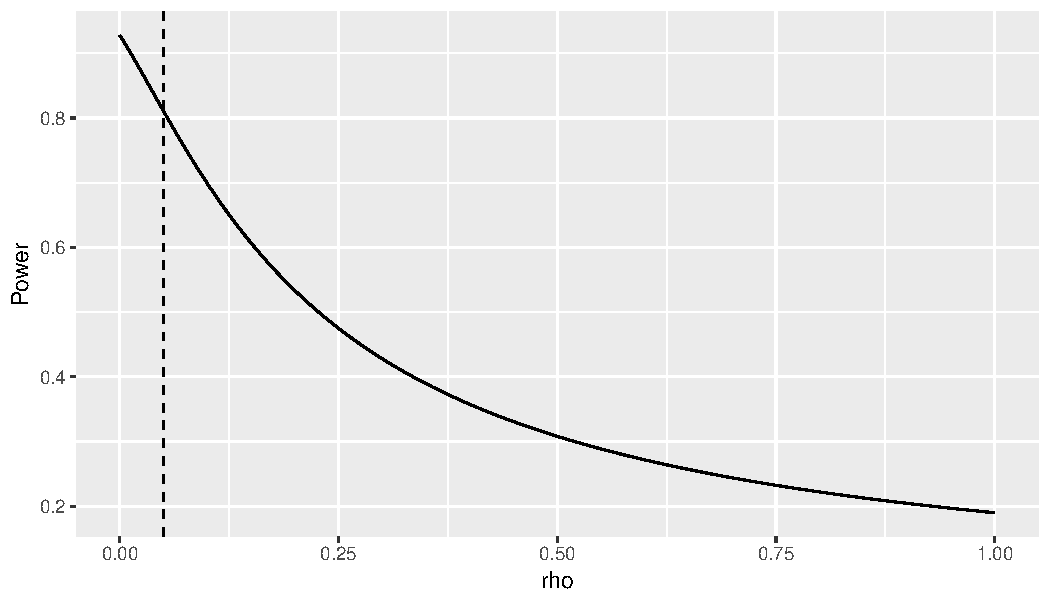
\includegraphics[scale=0.5]{power}
\end{frame}

\begin{frame}
\frametitle{Motivation}
For a fixed target power, a higher ICC will lead to a higher sample size requirement:
\begin{align*}
n &= n_{i}[1+(m-1)\rho^{*}] \\
n_{i} &= \text{sample size required when clustering is ignored}
\end{align*}
So, required sample size increases linearly with our chosen $\rho^{*}$.
\end{frame}

\begin{frame}
\frametitle{Practical solution}
\begin{example}[SHIFT]
``We anticipate that the level of clustering will be low for this particular trial - possibly around 0.01 but no higher than 0.05 \ldots assuming an ICC of 0.05 effectively reduces the power from 90\% to around 75\%. If the ICC were as low as 0.01, then this reduces the power to around 85\%.''
\end{example}
\end{frame}

\begin{frame}
\frametitle{Practical solution}
Trial design now considers another hypothesis:
\begin{align*}
\text{Minimise } & \text{sample size } n \\
\text{Minimise } & \text{type I error rate } \mid H_{0} \\
\text{Maximise } & \text{power } \mid H_{1}: \rho = 0.01 \\
\text{Maximise } & \text{power } \mid H_{2}: \rho = 0.05
\end{align*}
We down-weight the importance of $H_{2}$ compared to $H_{1}$ because we \emph{believe it to be less likely}, but we do this \emph{informally}.
\end{frame}

\begin{frame}
\frametitle{Practical solution}
\centering
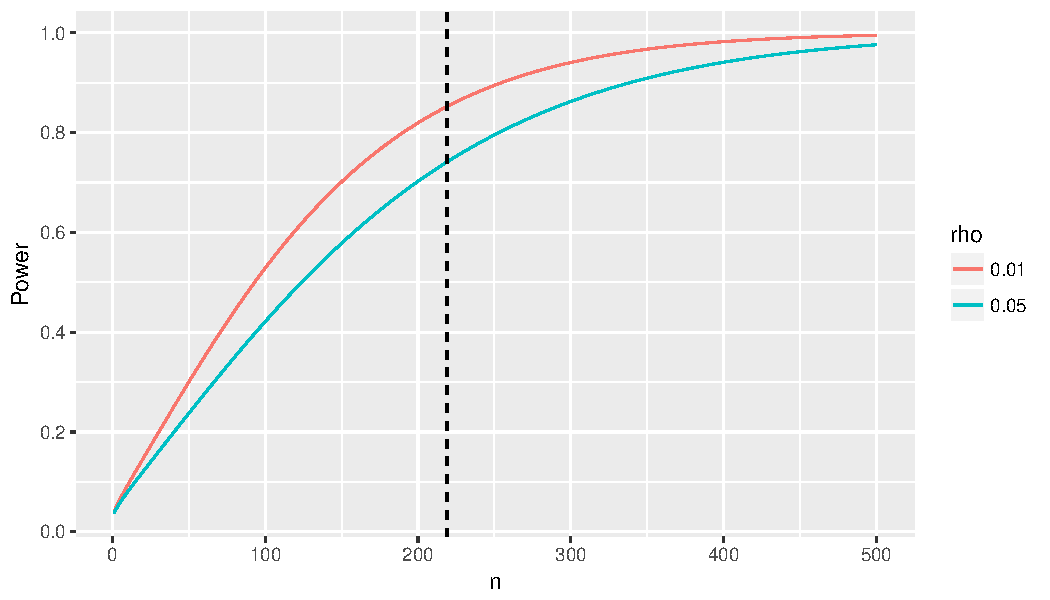
\includegraphics[scale=0.6]{power_2ICCs}
\end{frame}

\begin{frame}
\frametitle{Bayesian alternative}
An alternative: express our belief about the true value of $\rho$ using a probability distribution, e.g. $\rho \sim Beta(4, 58)$:\\
\vspace{3mm}
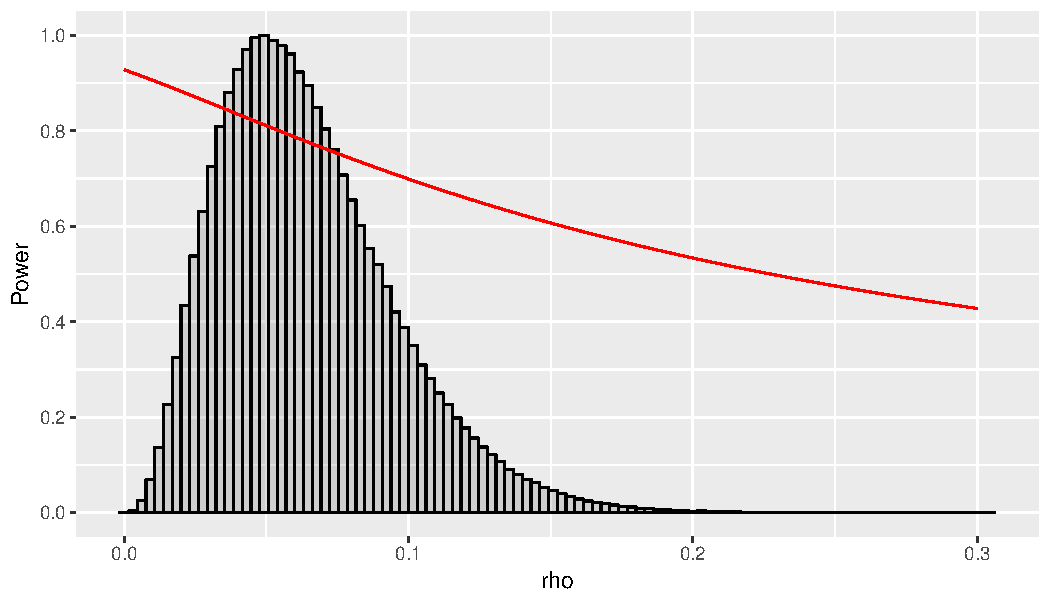
\includegraphics[scale=0.5]{prior_ICC}
\end{frame}

\begin{frame}
\frametitle{Bayesian alternative}
Should we use probability to express our uncertainty? Axioms\footcite{DeGroot1970}:
\begin{enumerate}
\item The relation $\succeq$, where $A \succeq B$ means $A$ is at least as likely as $B$, is a weak ordering (i.e. complete and transitive) on $S$.
\item If $A, B$ and $D$ are such that $AD = BD = \emptyset$, then $A \succeq B \Longleftrightarrow A \cup D \succeq B \cup D$.
\item $A \succeq \emptyset$ for any $A$. Furthermore, $S \succ \emptyset$.
\item If $A_{1} \supset A_{2} \supset \ldots$ is a decreasing sequence of events and $B$ is such that $A_{i} \succeq B$ for all $i$, then $\cap_{i=1}^{\infty} A_{i} \succeq B$.
\item There exists a random variable $X \sim Unif(0, 1)$.
\end{enumerate}
Together, these imply that there is a unique probability distribution $P$ that agrees with the relation $\succeq$.
\end{frame}

\begin{frame}
\frametitle{Bayesian alternative}
Uncertainty about $\rho \sim Beta(4, 58)$ propagates to uncertainty about power:\\
\vspace{3mm}
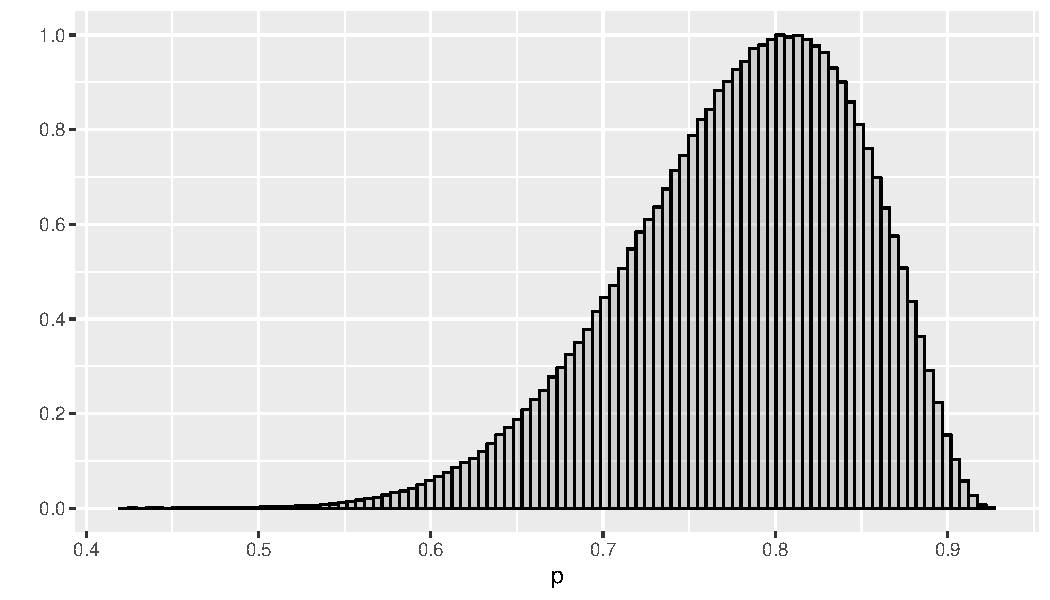
\includegraphics[scale=0.5]{prior_power}
\end{frame}

\section{Bayesian methods for trial design}

\frame{\tableofcontents[currentsection]}

\begin{frame}
\frametitle{Assurance}
Key paper: O'Hagan, Stevens and Campbell (2005), ``Assurance in clinical trial design'', \emph{Pharmaceutical statistics}.
\begin{itemize}
\item If event $A$ denotes a `successful' trial, and this is influenced by the true value of parameter(s) $\theta$, what is $Pr[A]$?
\item Unconditional, so we need to integrate out any parameters.
\end{itemize}
\begin{align*}
\text{assurance} = Pr[A] &= \int Pr[A \mid \theta]p(\theta) d\theta \\
 p(\theta) &= \text{probability density function of } \theta
\end{align*}
\end{frame}

\begin{frame}
\frametitle{Assurance}
\begin{example}[Unknown treatment effect]
For a two-sample comparison of normal means, suppose we are uncertain what the true treatment difference $\delta$ is. We think $\delta \sim N(0.2, 0.25^{2})$, and know that the common variance is $\sigma^{2} = 1$. Our trial has $n = 500$ in each arm, and will test at a level of $\alpha = 0.025$ (one-sided). What is $Pr[\text{reject } H_{0}]$?
\end{example}
\begin{enumerate}
\item Sample $\delta^{i} \sim N(0.2, 0.25^{2})$ for $i = 1, \ldots , N$
\item Calculate powers $\beta(\delta^{i})$
\item{ Compute the Monte Carlo estimate: 
	\begin{equation}
	Pr[\text{reject } H_{0}] \approx \frac{1}{N} \sum_{i=1}^{N} \beta(\delta^{i}) = 0.62.
	\end{equation}}
\end{enumerate}
\end{frame}

\begin{frame}
\frametitle{Assurance}
\begin{example}[Unknown treatment effect]
For a two-sample comparison of normal means, suppose we are uncertain what the true treatment difference $\delta$ is. We think $\delta \sim N(0.2, 0.25^{2})$, and know that the common variance is $\sigma^{2} = 1$. Our trial has $n = 500$ in each arm, and will test at a level of $\alpha = 0.025$ (one-sided). What is $Pr[\text{reject } H_{0}]$?
\end{example}
\begin{itemize}
\item Compare the unconditional power of 0.62 with the conditional power at $\delta^{*} = 0.2$ of 0.88.
\item Is this good enough? Should we adjust the sample size? 
\end{itemize}
\end{frame}

%- Optimality criteria, there are lots of metrics proposed but not much guidance on choosing the correct levels, makes sense since we need to trade-off quality against cost, advocated more generally in~\cite{Bacchetti2008}; minimising the number of patients per phase III success in~\cite{Stallard2012} is just choosing sample size at the steepest gradient of the unconditional power curve;
%Graph: unconditional power against n, highlighting Stallard solution and other potential trade-off gradiants

\begin{frame}
\frametitle{Optimality}
Given some measure(s) of the quality of a proposed trial design, how do we choose the best?
\begin{itemize}
\item Try to set some kind of standard threshold analogous to a power of 80\%.
\item Avoid thresholds and consider trade-offs~\footcite{Bacchetti2008};
\item Maximise performance per-patient~\footcite{Stallard2012};
\item Maximise expected utility~\footcite{Lindley1997}, possibly through an economic model~\footcite{Patel2013};
\end{itemize}
\end{frame}

\begin{frame}
\frametitle{Optimality}
\centering
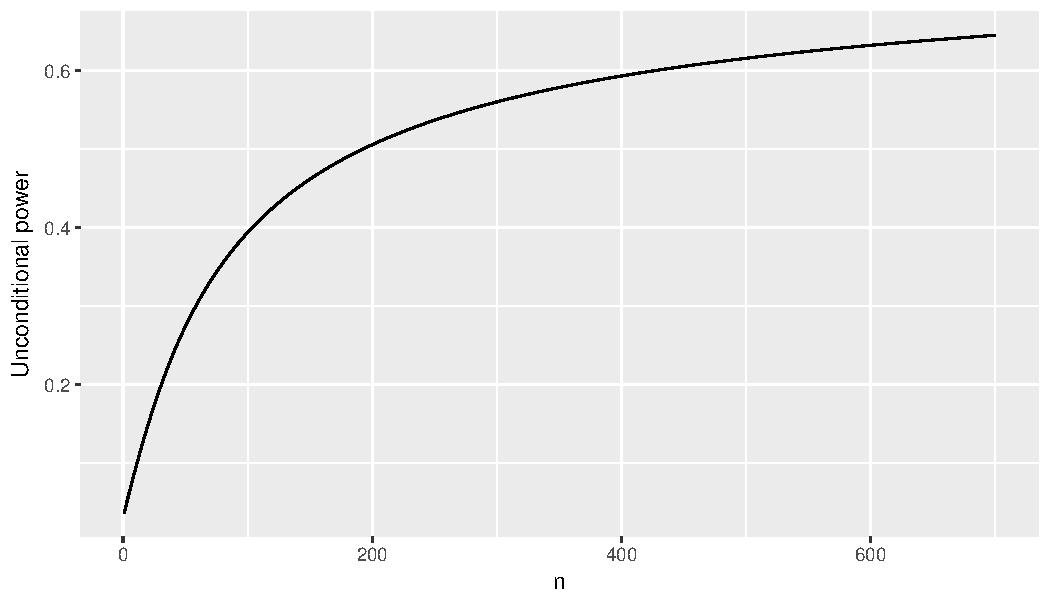
\includegraphics[scale=0.6]{stallard}
\end{frame}

%- Success criteria: probability of rejecting the null in two separate phase III trials~\cite{Zhang2013}; probability of an updated meta-analysis being positive~\cite{Sutton2007}; \cite{Walley2015} argue that unconditional power is not that useful, and argue for analogues of positive and negative predictive values;

\begin{frame}
\frametitle{Assurances}
The unconditional probability of rejecting the null hypothesis was the first hybrid Bayesian metric to be considered, but others have been proposed:
\begin{itemize}
\item Prob. rejecting the null \emph{and} the true effect being meaningful~\footcite{OHagan2005};
\item Prob. rejecting the null in \emph{two} separate phase III trials~\footcite{Zhang2013};
\item Prob. of a positive result in an updated meta-analysis~\footcite{Sutton2007}.
\end{itemize}
`Fully Bayesian' criteria have also been proposed:
\begin{itemize}
\item Prob. posterior probability the treatment effect is meaningful~\footcite{Ibrahim2014};
\item Conditional distribution of the treatment effect given a significant result~\footcite{Walley2015}.
\end{itemize}
\end{frame}

%- Uncertainty usually in treatment effects or typical nuisance parameters (sd's, ICC's, control group proportions), but some examples of more feasibility type considerations, e.g. sample size in each arm in~\cite{Ambrosius2010}, adherance rates in~\cite{Fay2006},

\begin{frame}
\frametitle{Uncertainty}
Various papers have addressed uncertainty in \ldots
\begin{itemize}
\item Treatment effects only~\footcite{OHagan2005};
\item Nuisance parameters only, including ICCs~\footcite{Turner2004} and parameters in survival models~\footcite{Ren2013};
\item Samples size~\footcite{Ambrosius2010};
\item Adherance rates~\footcite{Fay2006}.
\end{itemize}
For trials of complex interventions following a pilot we might also expect uncertainty in recruitment and data collection rates~\footcite{Avery2017}.
\end{frame}

%- Elicitation, particularly for parameters beyond just means and sd's or normal outcomes, e.g. parameters in survival models~\cite{Ren2014}, ICCs~\cite{Spiegelhalter2001}, and model structure  e.g. in a model of missing data.

\begin{frame}
\frametitle{Priors}
How do we define the priors to be used in these calculations?
\begin{itemize}
\item Using early phase trial data (empirical Bayes)~\footcite{Jiang2011};
\item Using other historical data, perhaps from a meta-analysis~\footcite{Sutton2007};
\item Using expert judgement~\footcite{Ren2013};
\item Using defaults, e.g. pessimistic and optimistic priors~\footcite{Spiegelhalter2004};
\item If using a fully Bayesian approach, consider differentiating between `design' and `analysis' priors~\footcite{Wang2002};
\end{itemize}
\end{frame}

%- Computation, back in~\cite{OHagan2006} they give some closed for expressions for the simplest cases and then use Bayesian clinical trial simulation for the more complex/realistic cases, and this patter is followed in a lot of subsequent work (in~\cite{Wang2013} they focus on only simulation note it can be used to get lots of other quantities e.g. expected study duration). Simulation definitely key to making the methods flexible, being Bayesian doesn't add any further computational burden to the usual approach if we are estimating a probability, although for other quantities it may lead to a higher variance and so more samples required, look into this. MC approach gets more intense as we move from simulating parameters and calculating power using a closed-form expression, to simulating trial test statistics, and finally to simulating trial data and computing the test statistics for these.
%Graph: EGO approach to sample size determination

\begin{frame}
\frametitle{Computation}
\begin{itemize}
\item Some papers focus on conjugacy~\footcite{Ibrahim2014};
\item The more flexible approach is through simulation~\footcite{Wang2013}, sampling test statistics if possible or failing that, individual patient data;
\item Bayesian (unconditional) simulation is no trickier than frequentist (conditional) simulation;
\item But simulation is time-consuming - if the design problem is complex, we need efficient optimisation methods.
\end{itemize}
\end{frame}

%- Interpretation issues come up a few times, e.g. in~\cite{Kirby2012} they talk about `true' and `theoretical' assurance, two point mass sampling priors are used in~\cite{Chen2011a} in an attempt (I think) to mimic frequentist operating characteristics, lots of papers (e.g.~\cite{Turner2004}) describe uncertainty in nuisance parameters but not in treatment effects, some try to avoid a Bayesian interpretation by viewing the distribution as one of the treatment effects of an (infinite) set of new treatments waiting to be evaluated~\cite{Goette2015} (similar to~\cite{Stallard2012}? short-run and long-run views), in~\cite{Kirchner2015} they define utility in terms of an estimated treatment effect rather than the true effect, uncertainty in variance is described in~\cite{Julious2006} as coming directly from the sampling distribution in a previous trial
%- A few papers talk about using the estimated treatment effect from a phase II study to design the phase III study, designing to detect that rather than an MCID (the papers tend to focus on the problems of the variability and the bias in this estimate). Is this common? Do we do it in Leeds? If so, why?

\begin{frame}
\frametitle{Interpretation}
\begin{itemize}
\item Can we have distributions for nuisance parameters but condition on treatment effects?~\footcite{Turner2004}
\item Can we have multiple priors?~\footcite{Chen2011a, Kirby2012}
\item Can we interpret a distribution of treatment effects from a frequentist perspective?~\footcite{Goette2015, Julious2006}
\end{itemize}
\end{frame}

\section{Bayesian designs for CI and pilot trials}

\frame{\tableofcontents[currentsection]}

\begin{frame}
\frametitle{Challenges}
\begin{itemize}
\item Complex models, e.g. recruitment, missing data, adherance, multilevel outcomes, multivariate outcomes~\footcite{Landau2013}
\item Complex design problem, e.g. multilevel sample sizes, multivariate acceptance regions, choice of primary endpoint
\item Qualitative gap between pilot and main trial settings, including changes to the intervention itself~\footcite{Hampson2017}
\item Computational burden of searching for optimal pilot designs~\footcite{Strong2015}
\end{itemize}
\end{frame}

\begin{frame}
\frametitle{Challenges}
\begin{itemize}
\item Complex models, e.g. recruitment, \textbf{missing data}, adherance, multilevel outcomes, multivariate outcomes~\footcite{Landau2013}
\item Complex design problem, e.g. multilevel sample sizes, multivariate acceptance regions, \textbf{choice of primary endpoint}
\item Qualitative gap between pilot and main trial settings, including changes to the intervention itself~\footcite{Hampson2017}
\item Computational burden of searching for optimal pilot designs~\footcite{Strong2015}
\end{itemize}
\end{frame}

\begin{frame}
\frametitle{Example}
\begin{example}[REACH(ish)]
One of the goals of out pilot study was to assess two potential primary outcomes for the main trial. We weren't sure about what treatment effects we might see, the variability in the outcomes, or how complete the data are likely to be. Following the pilot, a Bayesian analysis gives us posterior distributions on the relevant parameters.
\end{example}
\vspace{5mm}
\centering
\begin{tabular}{l l l l}
\toprule
Endpoint	& $\hat{\delta}$	& $\hat{\sigma}^{2}$	& $\hat{p}_{miss}$ \\
\midrule
A			& 0.145				& 1.16					& 0.75 \\
B			& 0.18				& 1.08					& 0.8 \\
\bottomrule
\end{tabular}
\end{frame}

\begin{frame}
\frametitle{Example}
\centering
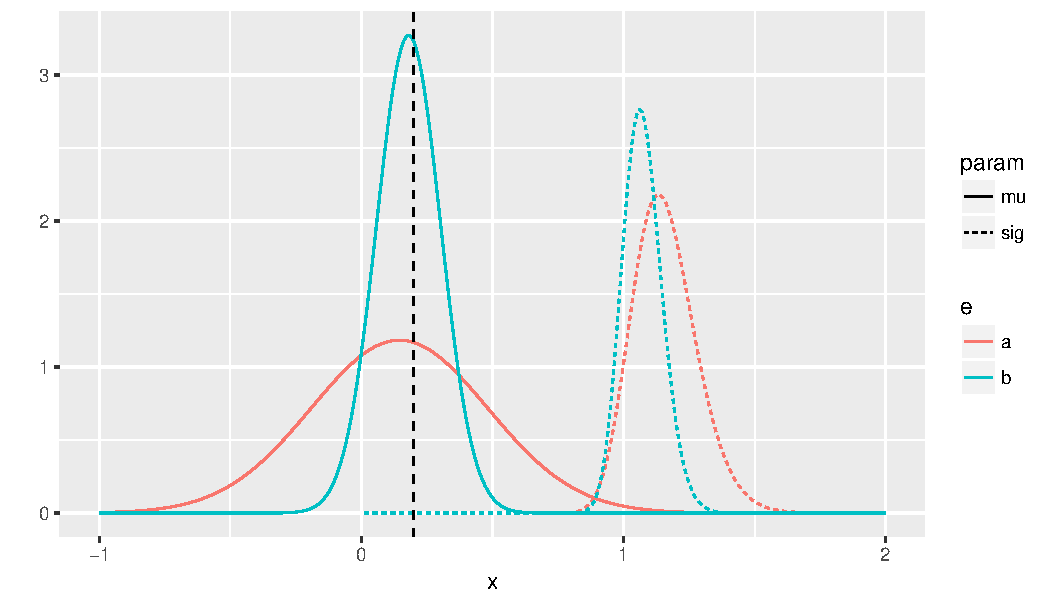
\includegraphics[scale=0.6]{endpoints1}
\end{frame}

\begin{frame}
\frametitle{Example}
\centering
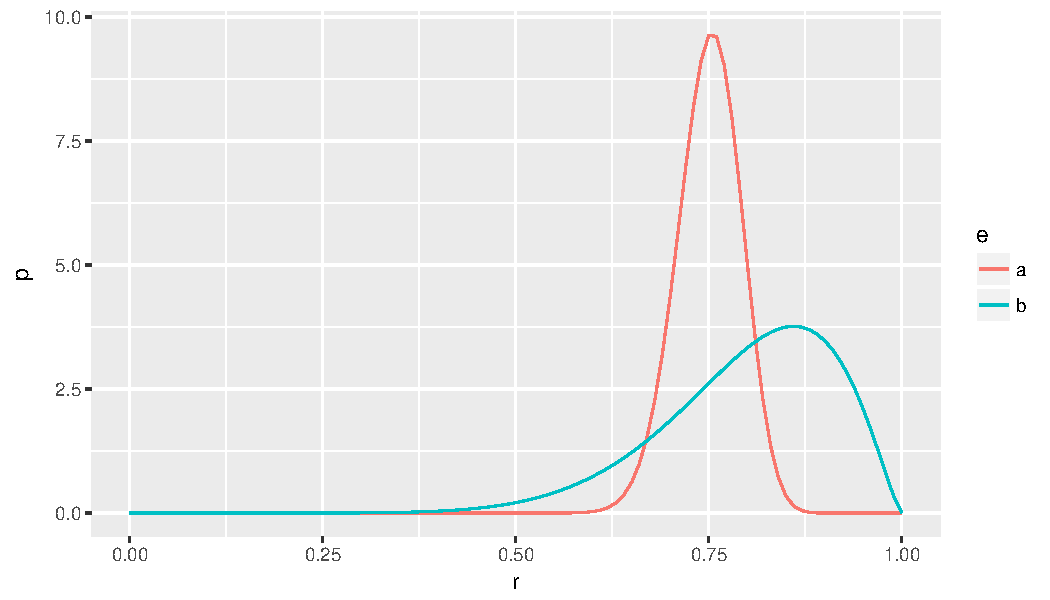
\includegraphics[scale=0.6]{endpoints2}
\end{frame}

\begin{frame}
\frametitle{Example}
\centering
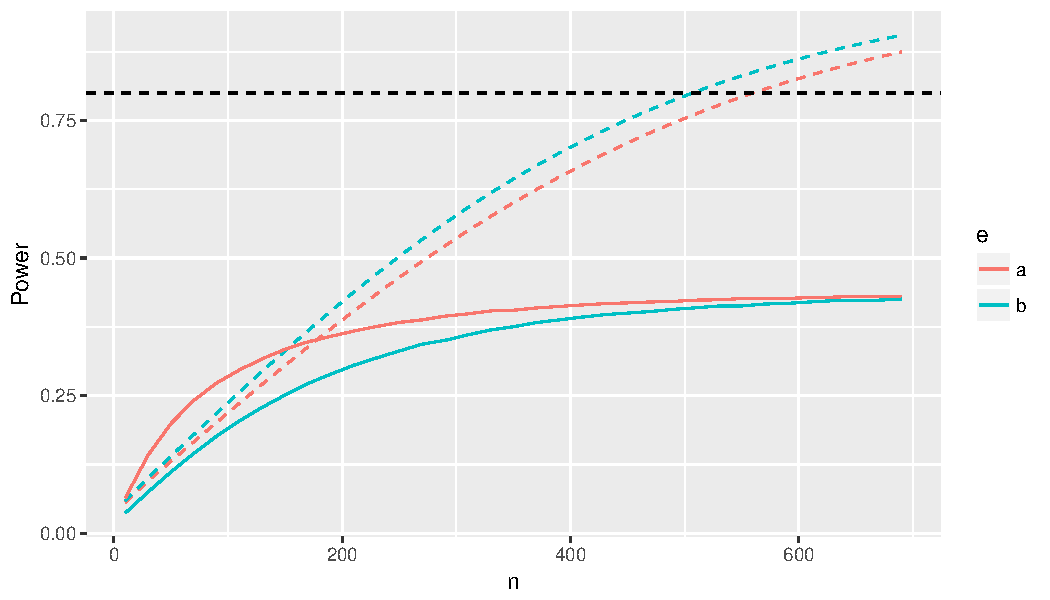
\includegraphics[scale=0.6]{endpoints3}
\vspace{1mm}
$510 \rightarrow 370$ patients per arm.
\end{frame}

\frame[allowframebreaks]{
\tiny
\printbibliography
}

\end{document}


